\documentclass[12pt,a4paper]{jarticle}
\usepackage[top=35truemm, bottom=35truemm, left=30truemm, right=30truemm]{geometry}
\usepackage[dvipdfmx]{graphicx}
\usepackage[version=3]{mhchem}
\setcounter{tocdepth}{\maxdimen} %subsubsectionまで目次を表示する
\bibliographystyle{junsrt} %参照のスタイル

\begin{document}
\begin{titlepage}
\title{\vspace{60mm} \LARGE 修士論文\vspace{10mm}\\J-PARC E07実験におけるbeam照射及び\\原子核乾板中の$\Xi$-粒子飛跡自動追跡}
\author{\Large 岐阜大学大学院 教育学研究科 \\ \vspace{5mm}
\Large 総合教科教育専攻 仲澤研究室 \\ \vspace{5mm}
\LARGE 後藤 良輔}
\date{最終更新 \today}
\maketitle
\thispagestyle{empty} %ページ番号を消す
\end{titlepage}

\thispagestyle{empty} %ページ番号を消す
\tableofcontents
\newpage
\section{序論}
\subsection{はじめに}
私たちを含め、身の回りの物質は原子からできている。
その原子核は原子核と電子から構成されており、原子核は陽子と中性子で成り立つ。
さらに、陽子や中性子はクォークで構成されている。
\par
クォークは、up(u)、down(d)、strange(s)、charm(c)、top(t)、bottom(b)の6種類がある。(以降は()内の文字で省略する。)
uとd以外のクォークを含む粒子は非常に寿命が短いため地球上に存在していない。
私たちはsクォークを含む粒子の相互作用について研究を進めている。
\par
一般に粒子の相互作用を調べるためには粒子同士の衝突散乱実験を行うが、上述した通りsクォークを含む粒子は寿命が非常に短いため衝突実験によって相互作用を知ることは不可能である。
例えば、私たちの研究で使用する$\Lambda$粒子はudsの3つのクォークからなり、その寿命は10$^-10$秒である。
そのため、$\Lambda$粒子の相互作用を求めるには原子核の中に$\Lambda$粒子持つものを生成し、核の崩壊過程から相互作用を求めるという手法しかない。
\subsection{Double-$\Lambda$Hyper核}
通常の核に$\Lambda$粒子を2つ持たせたものがDouble-$\Lambda$Hyper核である。
Double-$\Lambda$Hyper核を生成するため、K$^+$,K$^-$反応により$\Xi$$^-$粒子を生成する。
K$^+$,K$^-$反応は式(\ref{eq:K+-})の反応である。
そして、生成された$\Xi$$^-$粒子を原子核に吸収させることで式(\ref{eq:Xi_eq})の反応を起こし$\Lambda$粒子を生成する。
\begin{equation}
	\ce{K- + p -> $\Xi$- + K+}
\label{eq:K+-}
\end{equation}
\begin{equation}
	\ce{$\Xi$- + p -> $\Lambda$ + $\Lambda$ + 28.6Mev}
\label{eq:Xi_eq}
\end{equation}
\par
E07実験では、K$^-$粒子を生成しDiamond Targetに照射することで$\Xi$$^-$粒子を生成する。
そして、生成された$\Xi$$^-$粒子を原子核乾板中で静止させる。
$\Xi$$^-$粒子は電離損失により$\Xi$$^-$粒子の持つエネルギーが減少していく。
エネルギーが減少した後に乾板中の原子核に吸収されることで、核内の陽子と反応を起こす。
これらの反応により生成された2つの$\Lambda$粒子が原子核の中にとどまると、Single-$\Lambda$Hyper核やDouble-$\Lambda$Hyper核が生成される。
\par
E07実験では上述したとおり原子核乾板の外で$\Xi$$^-$粒子を生成し、乾板中で$\Xi$$^-$粒子を反応させる。
しかし、それ以外にもK$^-$粒子が原子核乾板の中の原子核と反応しDouble-$\Lambda$Hyper核ができる場合もある。
\par
\begin{figure}[htbp]
    \begin{center}
     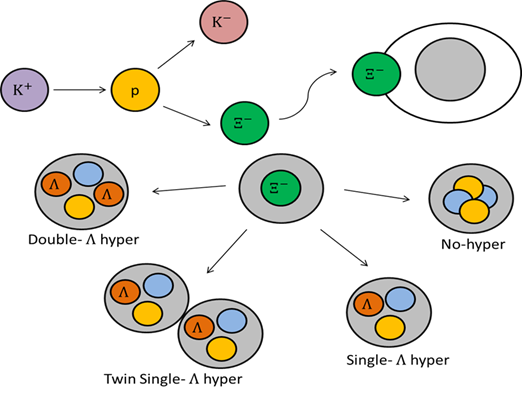
\includegraphics[width=120mm]{makehyper.png}
    \end{center}
    \caption{Hyper核生成過程\label{fig:makehyper}}
   \end{figure}
\newpage
\subsection{原子核乾板}
原子核乾板とは非常に高感度な写真フィルムの一種で、荷電粒子の通過した跡を記録する検出器である。
私たちが実験で使用する$\Lambda$粒子の寿命は非常に短いため、Hyper核の生成・崩壊事象をすべて記録できる原子核乾板を使う必要がある。
\par
原子核乾板の利点としては大きく分けて2点ある。
\par
一点目は、現像処理を行うことで半永久的に顕微鏡による観測を可能にすることである。
原子核乾板中を荷電粒子が通ることで、原子核乾板の主成分であるAgBrが電離され銀原子が生成される。
現像処理により、銀が成長し1µm程度の粒となり(grain)、荷電粒子の飛跡がgrainの連なり(飛跡、track)として現れ、その状態を保持する。
そのため、原子核乾板を破損しない限り一度記録したHyper核の生成・崩壊事象やHyper核以外の荷電粒子秘跡を何度でも同じ状態で観測することができる。
\par
\begin{figure}[htbp]
    \begin{center}
     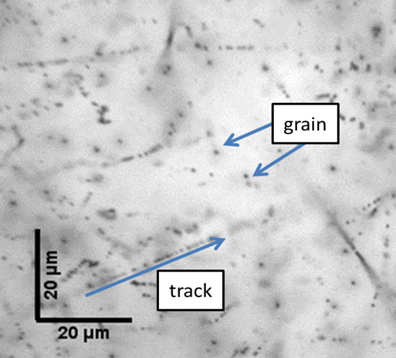
\includegraphics[width=70mm]{grainfog.png}
    \end{center}
  \caption{原子核乾板中に飛跡が記録される流れ\label{fig:process_recored_track}}
\end{figure}
\begin{figure}[htbp]
 \begin{center}
  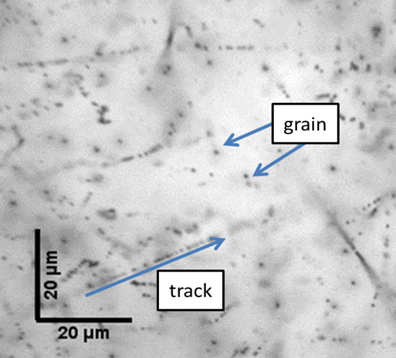
\includegraphics[width=70mm]{grainfog.png}
 \end{center}
 \caption{原子核乾板中に記録されるtrackとgrainの様子\label{fig:grain_track}}
\end{figure}
二点目は、サブミクロン精度での空間分解能を持つことである。
生成される銀粒子の大きさがμmオーダーのため、その大きさでの位置分解能が出る。
また、乾板に記録された飛跡の長さ、太さは通過した荷電粒子のエネルギーや電荷に依存する。
そのため、私たちは記録されたHyper核事象の飛跡の長さと角度からエネルギーを計算することで$\Lambda$-$\Lambda$間に働く相互作用を算出することができる。
\par
原子核乾板はBaseにEmulsionを塗布して作成している。
Baseとはポリスチレンフィルムで作られた支持体である。
Emulsionは通常の写真乳剤よりもハロゲン化銀の含有量が高く,最小電離損失に対して感度を持っているものである。
E07実験で使用する原子核乾板1400枚(薄型:200、厚形:1200)はすべて岐阜大学で製造された。
\par
E07実験で使用する乾板は40µmのBaseに450µmの乳剤を塗布する厚型乾板と、180µmのBaseに100µmの乳剤を塗布する薄型乾板の二種類である。
\par
薄型乾板はSSDとemulsionとの接続に使用される。
薄型乾板はbaseが厚く、乳剤が薄く塗布されているため現像の前後で乾板の変形が小さい。
そのため、記録された飛跡の角度や位置を明確に求められる。
\par
厚形乾板は照射された$\Xi$粒子を乾板中で静止させ、娘粒子の飛跡を記録するために用いられる。
\par
\begin{figure}[htbp]
    \begin{center}
     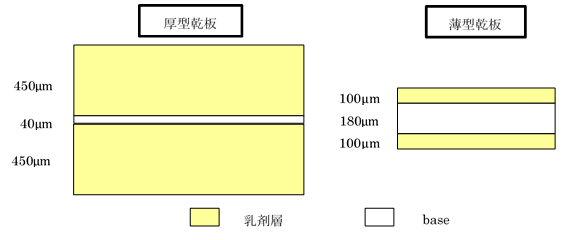
\includegraphics[width=140mm]{emulsionorder.png}
    \end{center}
    \caption{使用する原子核乾板の規格\label{fig:emulsionorder}}
\end{figure}
\subsection{光学顕微鏡}
光学顕微鏡を用いて、現像後の原子核乾板に記録されているtrackを追跡、観察する。
使用する顕微鏡は、モーターによって水平方向(x、y方向)に約1µmの精度で位置制御し、エンコーダーによって鉛直方向(z方向)に約0.1µmの精度で稼働できる。
この顕微鏡により、原子核乾板表面の推測される位置で目的のtrackを探し、$\Xi$$^-$粒子候補を見つけ、trackを原子核乾板上面から下面まで追跡していく。
\par
PCを接続することで、この光学顕微鏡を制御している。CCDカメラを顕微鏡に設置することで、顕微鏡で観察したものを画像として取得する。
取得した画像をPCの画面上に表示することや、顕微鏡の稼働に活用している。
$\Xi$$^-$粒子自動追跡には、50倍の対物レンズを使用している。
\begin{figure}[htbp]
    \begin{center}
     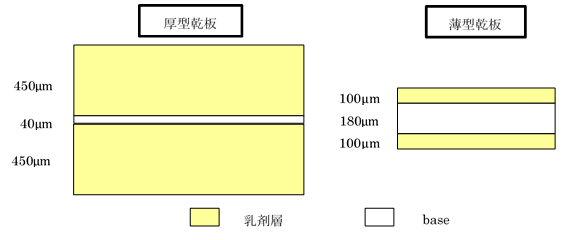
\includegraphics[width=140mm]{emulsionorder.png}
    \end{center}
    \caption{光学顕微鏡\label{fig:microscope}}
\end{figure}
\newpage
\subsection{KEK-PS E373実験}
E373実験はE176実験に続くDouble-$\Lambda$Hyper核検出実験である。
\cite{Nagara}
\cite{Nagara2}
E176実験の約10倍のDouble-$\Lambda$Hyper核の検出を目標にし、エマルジョンとカウンターを組み合わせたハイブリッド-エマルジョン法を取り入れて実施された。
約1000の$\Xi$$^-$粒子吸収事象が見積もられ、光学顕微鏡を用いた半自動飛跡追跡により全モジュールの解析が終了している。
解析の結果、約600例の$\Xi$$^-$粒子吸収事象を検出し、7例のDouble-$\Lambda$Hyper核を検出した。
その中の1例でのみ崩壊モードを一意に決定することができ、この1例をNAGARA Eventと名付けた。
\begin{figure}[htbp]
    \begin{center}
     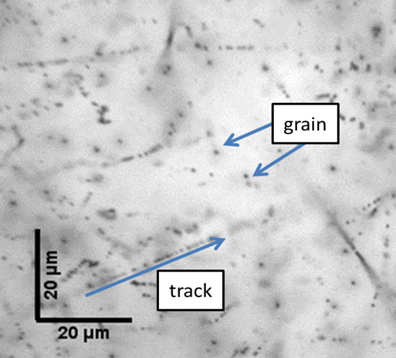
\includegraphics[width=70mm]{grainfog.png}
    \end{center}
    \caption{Nagara eventとKiso event\label{fig:Nagara_Kiso}}
\end{figure}
\subsection{J-PARC E07実験}
J-PARC E07実験はハイブリッド-エマルジョン法によりKEK-PS E373実験の10倍の統計量を目指す実験である。
表\ref{tab:compare_E07_E373}はJ-PARC E07実験とKEK-PS E373実験の比較をしたものである。
表にあるように、beamのK$^-$/$\pi$$^-$を約3.5倍、原子核乳剤の量を約3倍にすることで10倍の$\Xi$$^-$粒子静止事象を実現する。
\par
SSDは電荷をもった粒子が通過した際に、通過した粒子が原子核乾板スタックのどの位置にどのような角度で照射されているかの情報を記録するものである。
原子核乾板スタックを2つのSSDで挟むことで、Diamond Targetで生成された$\Xi$$^-$粒子だけでなく、原子核乾板内で反応した$\Xi$$^-$粒子の情報も記録できる。
SSDの情報を使い、emulsionに記録された飛跡の中で$\Xi$$^-$粒子である確率の高い飛跡のみを追跡することでいち早くDouble-$\Lambda$Hyper核を検出する。
SSDの精度と前回の検出器の精度の違いを示す。
これがハイブリッド-エマルジョン法である。
\begin{table}[htbp]
\centering
\caption{J-PARC E07実験とKEK-PS E373実験の比較\label{tab:compare_E07_E373}}
\begin{tabular}{c|c|c}
   &KEK-PS E373実験&J-PARC E07実験\\
\hline
\hline
$\Xi$$^-$粒子静止事象 & ~10$^3$    & ~10$^4$  \\
K$^-$/$\pi$$^-$ & 1/4  & 6/1 \\
原子核乳剤量 & 0.8t & 2.1t  \\
\hline
\end{tabular}
\end{table}
\begin{table}[htbp]
\centering
\caption{原子核乾板中に記録されるtrackとgrainの様子\label{tab:grain_track}}
\begin{center}
    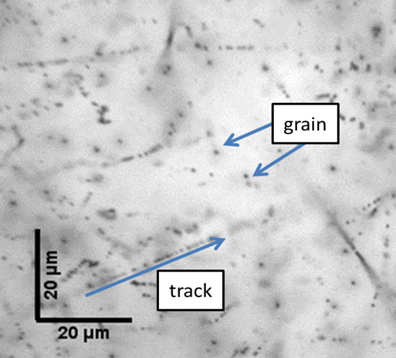
\includegraphics[width=70mm]{grainfog.png}
\end{center}
\end{table}


\newpage
\section{J-PARC E07実験2ndRun}
J-PARC E07実験は1stRunを2016年6月18日〜30日に、2ndRunを●~●に実施した。
1stRunでは18stacks、2ndRunでは100stacksのbeam照射に成功した。
beam照射を行うにあたり使用する原子核乾板のバックグラウンド削減法の実施、原子核乾板の真空パック法の確立、現像等を実施した。
\par
本章ではJ-PARC E07実験beam照射、現像においての実施内容及びその手法について述べる。
\subsection{Refresh処理の実施}
\subsubsection{実施背景}
\begin{itemize}
 \item 放射能漏れで乾板を制作した直後にbeam照射ができなかった。
 \item 莫大なバックグラウンドの増加を防ぐため神岡鉱山内にて制作した原子核乾板を保管
 \item 神岡内で保管したことで岐阜大で保管するよりバックグラウンドの増加を押さえることができた。
 \item しかし、解析に支障が出る程度まで蓄積されたため、リフレッシュ処理を実施した。
 \item E07実験では1stRunで●枚、2ndRunで●枚のリフレッシュ処理を実施した。
\end{itemize}
J-PARC E07実験で使用する原子核乾板はすべて岐阜大学ダブルハイパー核実験棟にて制作した。
制作は2013年12月~2014年3月の期間で完了している。
当初の予定では乾板製造後すぐにbeam照射を実施する予定であったが、J-PARCでの放射能漏れ事故により実験は延期になった。
\par
製造した原子核乾板は現像されるまで空気中の宇宙線やコンプトン電子を記録していく。
これらのバックグラウンドが増加すると、beam照射後の解析に支障を来す恐れがある。
そこで、宇宙線の影響が少ない神岡鉱山内に鉛ブロックで箱を作り、製造した原子核乾板を保管した。
\par
図\ref{fig:compton_and_cosmicray_in_emulsion}は製造からの時間経過による原子核乾板記録された宇宙線、コンプトン電子の増加稽古を示している。
赤色が岐阜大学の冷蔵庫内で保管した場合、青色が神岡鉱山鉛箱内で保管した場合である。
二つの線の傾きを比較すると、神岡鉱山内で保管したことで非常に多くのバックグラウンドを削減することができたということが分かる。
\par
しかし、製造からbeam照射まで2年の期間が経過したため、神岡鉱山内で保管していたとしても解析に支障を及ぼすレベルまでバックグラウンドが蓄積してしまった。
図\ref{fig:beam_efficiency_to_compton}はコンプトンの蓄積量に対するbeam検出効率を示したものである。
図からbeam検出効率が著しく低下することが分かる。
また、図\ref{fig:britnese_in_some_emulsion}はバックグラウンド蓄積量の違う乾板での輝度値の位置変化を示している。
図からバックグラウンドの増加により、コントラストが悪くなることが分かる。
\par
これらのことから、蓄積されたバックグラウンドの消去のために原子核乾板に対して潜像退行処理(Refresh処理)を実施した。
\par
\begin{figure}[htbp]
    \begin{center}
     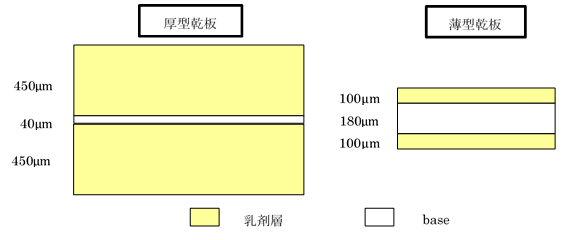
\includegraphics[width=140mm]{emulsionorder.png}
    \end{center}
    \caption{乾板に記録されたコンプトンと宇宙線\label{fig:compton_and_cosmicray_in_emulsion}}
\end{figure}
\begin{figure}[htbp]
    \begin{center}
     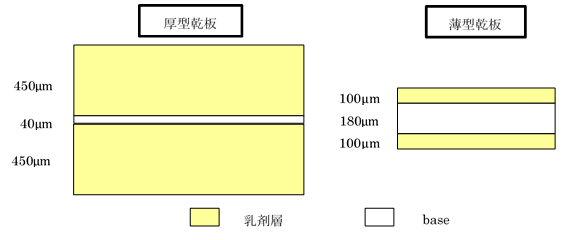
\includegraphics[width=140mm]{emulsionorder.png}
    \end{center}
    \caption{神岡鉱山内の鉛ブロック中に原子核乾板の保管状況\label{fig:emulsion_in_Kamioka}}
\end{figure}
\begin{figure}[htbp]
    \begin{center}
     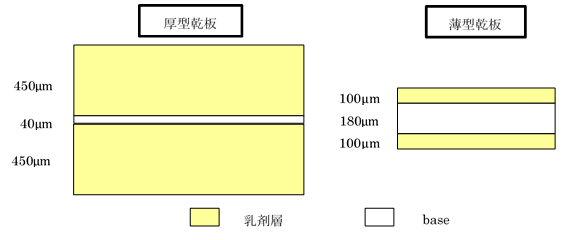
\includegraphics[width=140mm]{emulsionorder.png}
    \end{center}
    \caption{コンプトンの蓄積量に対するbeamの検出効率\label{fig:beam_efficiency_to_compton}}
\end{figure}
\begin{figure}[htbp]
    \begin{center}
     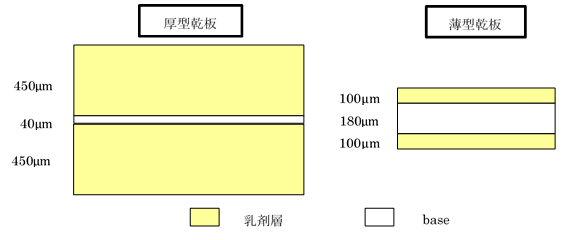
\includegraphics[width=140mm]{emulsionorder.png}
    \end{center}
    \caption{バックグラウンド蓄積量の違う乾板での輝度値の位置変化\label{fig:britnese_in_some_emulsion}}
\end{figure}
\subsubsection{原理}
\begin{itemize}
 \item 写真乾板には潜像退行性がある。
 \item 高温・多湿の環境下に乾板を置くことでその性質を促進し記録されたバックグラウンドを消去することを潜像退行処理という。
 \item たくさんのD論も引用でいれるか。
\end{itemize}
写真フィルムには撮影してから現像するまでに時間を経ると、映像が消えていく性質(潜像退行性)がある。
また、潜像退行性は高温高湿度の環境で著しく進むことが明らかになっている。
\par
原子核乾板は塗布されてから現像されるまでの間に、自然放射線や宇宙線の影響を受け潜像が蓄積される。
そこで、蓄積された潜像を消去するための手法として潜像退行処理(Refresh処理)と呼ばれる方法が開発されている。
\cite{takusann}
\par
\subsubsection{実施環境}
\begin{itemize}
 \item リフレッシュ処理を行うには温度●度、湿度●%の環境を●時間維持する必要がある。
 \item リフレッシュ処理を行うためその環境を維持する装置を作成した。
 \item 1stRunでは温度・湿度の調整を手動で行ってきたが、2ndRunでは温度・湿度の調整を自動で制御させた。[村本卒論]
 \item 湿度と厚みのグラフを載せて制御できていると書く。
\end{itemize}
\subsubsection{評価}
\begin{itemize}
 \item リフレッシュ処理の実施によりバックグラウンドが減少した。[大橋卒論]
 \item 1stRun、2ndRunのリフレッシュ処理の評価&最適化の詳細は大橋修論にて述べる。
\end{itemize}
\subsection{GridMark照射環境の最適化}
\subsubsection{暗室の拡張}
1stRunではbeam照射後の原子核乾板を岐阜に持ち帰り、現像の数日前に岐阜でGridマークを照射した。
これが原因であるかは分からないが、Gridマークの位置ズレが一様でなかったため一視野内に飛跡を持ってくることが困難になった。これいらないかも…
2ndRunではbeam照射後の原子核乾板に対してJ-PARC内の暗室下でGridMark照射を実施した。
そのため、2017年3月にGridMark照射装置を設置するため暗室の拡張を行った。
\par
図●は拡張前、図●は拡張後の暗室を示したものである。
横の長さを1m拡張することで、Gridマーク照射装置を設置する場所を確保した。
図として実際の内部の図を入れる。
\subsubsection{GridMarkネガ}
2016年にE07実験testRunにてbeam照射を実施した。
その際、原子核乾板に焼き付けられたGridマークはネガのつまりにより場所により照射されていないものが存在していた。
1stRunのGridマーク照射の際は図●の装置を使用してネガのつまりを解消した上で照射を行った。
しかし、1stRunの原子核乾板においてもGridマークが照射されていない箇所が存在した。
\par
これらを受けてネガの変更を行った。E07実験のと同様に発注し、ネガを貼り付けた。
図として発注したネガの図を示す。(くずやの測定した図でも良いかもしれん)
\subsubsection{GridMark照射装置}
\begin{itemize}
 \item 1stRun乾板は人がストップウォッチを使い、10秒間露光すると言うことを●枚の乾板に対して実施した。
 \item この手法では1mod分照射するのに●時間が必要になるとともに、精神的疲労が大きいので変更した。
 \item 一瞬で●rpm?露光できるように作り替えた。
 \item 装置はこんな感じである。
\end{itemize}
E071stRunではタイマーを用いて10秒間原子核乾板に露光した。
(田村卒論)参照論文と同様の手法で1mod分照射するのに約1時間半の時間が必要になるとともに時間をストップウォッチを使って計測していたため、多大な精神的疲労を負うことになっていた。
E07実験2ndRunではbeam照射後すぐにGridマークを照射する。
従来の手法から変更することで照射の時間短縮及び疲労の削減のために照射装置の改造を行った。
\par
田村卒論を確認して、露光時間、最終的にどれくらい照射すれば良いのか、照射装置の構造の写真を引用して載せる。
\par
吉田氏が組んだ回路の図を載せる。
田村さんの卒論からGridマークを焼き付けるのにどれくらい照射する必要があるのかを確認して引用する。
\subsection{E07実験beam照射}
\subsubsection{2ndRunbeam照射}
\begin{itemize}
 \item ●日をかけて原子核乾板●枚すべてにbeam照射を行った。
 \item beamライン等の図。Runendの図を見せて終了。
 \item 何日かけて実施したかを記す。照射Mod数/月日 の図
\end{itemize}
2017年5月●日~7月●日にかけて100stacksの原子核乾板すべてにbeam照射を行った。
\subsubsection{作業内容}
ここではemulsionカセットに乾板を詰める作業と乾板をカセットから出す。
作業について書く。
\par
遠藤修論を参考文献にする。
\begin{itemize}
 \item 乾板を冷蔵庫から出す。
 \item 袋から乾板を開けて乾板の重さ・厚さを測定し、乾板の番号を記録、乾板のMOD番号を書く。
\end{itemize}
暗室内で原子核乾板をEmulsionCasetteに詰める際の流れは以下の通りである。
\begin{enumerate}
    \item 冷蔵庫で保管されていた原子核乾板をパッキングする数時間前に暗室下に出し、温度に慣らす。
    \item グリスを塗った、Oリングをはめ込む。
    \item カセットの4つ角にL字のSUS板を置く。 
    \item 原子核乾板を袋から出し、乾板の番号を確認する。
    \item Mod、pl番号を原子核乾板の右下に記入する。
    \item シックネスゲージを使い、乾板の四点の厚さを測定する。
    \item 乾板の重さを測定する。
    \item 乾板をSUS板に沿って原子核乾板13枚をカセットに入れる。
\end{enumerate}
\subsubsection{EmulsionCasetteでの真空度}
\begin{itemize}
 \item 遠藤修論にある基準をクリアすることを確認しながら実施。
 \item ある真空度グラフをのせ、適切に行えたということを示す。
 \item 残りのModに関しては付録にあると記す。
\end{itemize}
\subsubsection{EmulsionCasetteの固定法確立}
\begin{itemize}
 \item 遠藤修論にあるカセットを押さえる装置を2ndRunでは導入して実施した。
 \item 1stRunでは●回で●回SUSを張り直していたが、2ndRunでは●回で1度しかSUSを張り直さなかった。
\end{itemize}
\subsubsection{照射した乾板の密度}
\begin{itemize}
 \item カセットに入れる前と後で重さが大きく変化していないかを確認した。
 \item 測定した重さと厚さから乾板の密度を求めたところ、1stRunと2ndRunで密度の大きな違いは無かった。リフレッシュ処理の有無も乾板の密度測定には影響がなかったと言える。
\end{itemize}
2ndRunでは1stRunと同様にemulsionCasetteに乾板を入れる前に乾板の厚さと重さの測定、beam照射後に乾板の重さを測定することでbeam照射により乾板の重さに大きな変動がないかを確認した。
照射の前後で重さが1.0g以上異なっていた場合再度厚さ重さの測定をして記録した。
乾板の重さは電子天秤を用いて、乾板の厚さはシックネスゲージを用いて乾板の4カ所を測定した。
\par
使用した電子天秤とシックネスゲージの写真
\par
図\ref{fig:compare_thick_den}は厚形乾板の1stRun乾板での密度の測定結果と2ndRun乾板での密度の測定結果である。
比較すると、1stRunと2ndRunで使用した原子核乾板に大きな違いは無いように見える。
また、1stRun乾板の密度はRefresh未処理の乾板、2ndRunはRefresh実施乾板での密度である。
そのため、Refresh処理の有無で原子核乾板の密度が変化しないことが分かる。
\par
薄型乾板でも同様に密度の比較をした。
図\ref{fig:compare_thin_den}を見ると、1stRunの薄型乾板は厚形乾板より密度が大きく算出されていたが、2ndRunで使用した薄型乾板でも同様の傾向になった。
\begin{figure}[htbp]
    \begin{center}
      \begin{tabular}{c}
        % 1枚目の画像
        \begin{minipage}{0.5\hsize}
          \begin{center}
            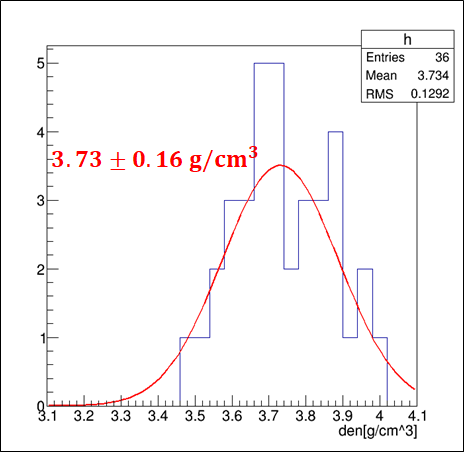
\includegraphics[clip, width=60mm]{1stRun_thin_den.png}
            \hspace{1.6cm} (a)1stRun 厚形乾板密度 可塑剤6.0cc
          \end{center}
        \end{minipage}
        
        % 2枚目の画像
        \begin{minipage}{0.5\hsize}
          \begin{center}
            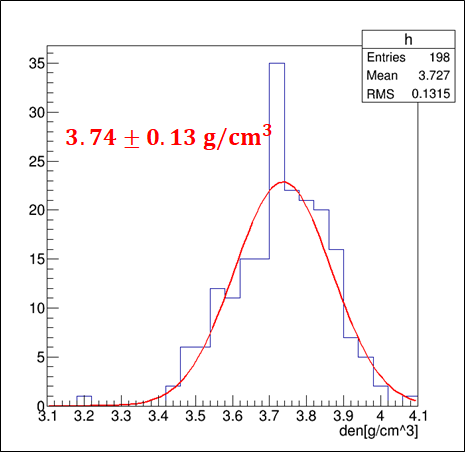
\includegraphics[clip, width=60mm]{2ndRun_thin_den.png}
            \hspace{1.6cm} (b)2ndRun 厚形乾板密度 可塑剤6.0cc
          \end{center}
        \end{minipage}\\

	 \\
        % 3枚目の画像
        \begin{minipage}{0.5\hsize}
            \begin{center}
              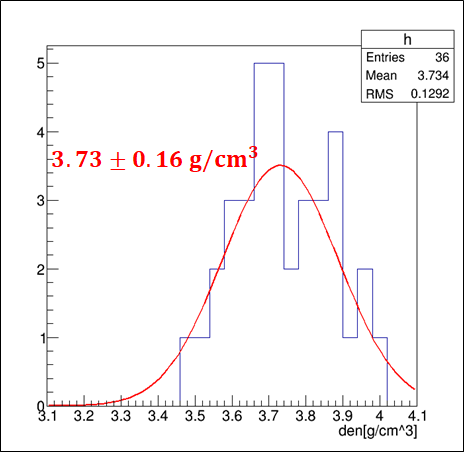
\includegraphics[clip, width=60mm]{1stRun_thin_den.png}
              \hspace{1.6cm} (c)1stRun 厚形乾板密度 可塑剤7.5cc
            \end{center}
          \end{minipage}
          
        % 4枚目の画像
        \begin{minipage}{0.5\hsize}
            \begin{center}
              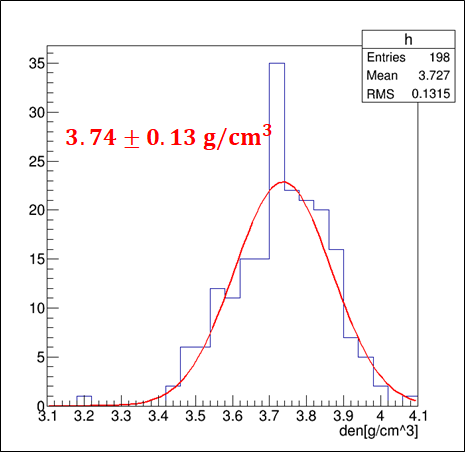
\includegraphics[clip, width=60mm]{2ndRun_thin_den.png}
              \hspace{1.6cm} (d)2ndRun 厚形乾板密度 可塑剤7.5cc
            \end{center}
        \end{minipage}
    
      \end{tabular}
      \caption{厚形乾板の密度比較\label{fig:compare_thick_den}}
    \end{center}
\end{figure}
\begin{figure}[htbp]
    \begin{center}
      \begin{tabular}{c}
        % 1枚目の画像
        \begin{minipage}{0.5\hsize}
          \begin{center}
            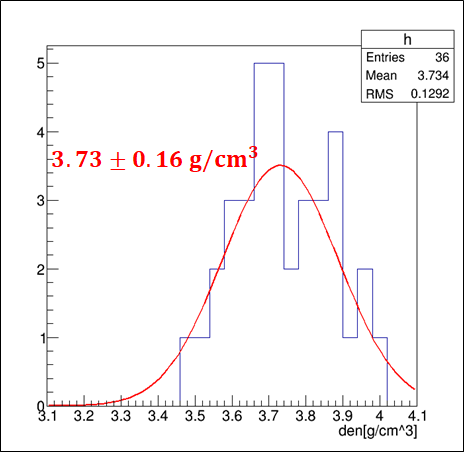
\includegraphics[clip, width=60mm]{1stRun_thin_den.png}
            \hspace{1.6cm} (a)1stRun 薄型密度
          \end{center}
        \end{minipage}
        
        % 2枚目の画像
        \begin{minipage}{0.5\hsize}
          \begin{center}
            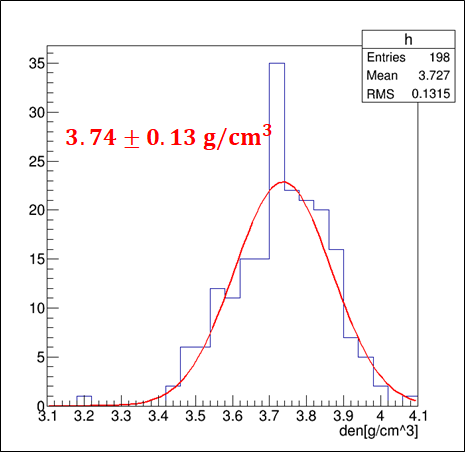
\includegraphics[clip, width=60mm]{2ndRun_thin_den.png}
            \hspace{1.6cm} (b)2ndRun 薄型密度
          \end{center}
        \end{minipage}
    
      \end{tabular}
      \caption{薄型乾板の密度比較\label{fig:compare_thin_den}}
    \end{center}
\end{figure}
\newpage
\subsection{現像}
\begin{itemize}
 \item 原子核乾板すべて現像している。
 \item 現像の行程
 \item 1stRunは●年に●枚終了、2ndRunは●年に●枚終了予定
 \item 現像の詳細な記述は大橋修論に記載する。
\end{itemize}
\subsubsection{原理}
\subsubsection{実施環境}
\subsubsection{評価}

\newpage
\section{荷電粒子飛跡追跡の自動化}
\subsection{目的}
E373実験では人が約2.0×10$^4$本の$\Xi$$^-$候補を顕微鏡を使い静止点まで追跡した。
この追跡には約数年が必要となった。
先に記述したが、今年度実施されたJ-PARC E07実験ではハイブリッド-エマルジョン法によりE373実験の約10倍の統計量を検出することを目標にしている。
今回実施されたE07実験では、E373実験より精度の高い検出機であるSSDを使うことで追跡するべき飛跡を増やさないようにしている。
しかし、その条件であっても追跡すべき$\Xi$$^-$候補飛跡はE373実験を超えるため、機械が自動で飛跡を静止点まで追跡するプログラムが必要になった。
\par
この章では$\Xi$$^-$候補飛跡のために開発した要素技術について記述する。
SSDとE373実験の際に使用された検出機の精度をまとめた表を示す。
\subsection{$\Xi$$^-$候補&beam認識に用いる画像処理}
\subsubsection{コントラスト処理}
\begin{itemize}
    \item 乾板の写真は撮影した地点によりコントラストが異なるので、撮影の位置によらず画像を同等に扱いたいのでコントラスト処理をかける。
    \item 位置による乾板中の飛跡の見え方の違いを示す。
    \item コントラスト処理で使用する数式を示す&それを説明した図を入れる。
    \item 処理前と処理後の画像を入れる。
\end{itemize}
原子核乾板中を撮影した画像は、画像を撮影した原子核乾板の位置により見え方が異なる。
図●は同一乾板内で撮影した写真で、視野中心に見えるのは追跡対象にしている$\Xi$$^-$候補飛跡である。
二つの写真の違いは原子核乾板の位置で、左が上側乳剤層、右が下側乳剤層で撮影したものである。
図より撮影地点が異なれば画像のコントラストが大きく異なることが分かる。
そこで、原子核乾板中で撮影した画像に記録された飛跡情報を的確に取得するために画像のコントラストの違いをなくす必要がある。
\begin{figure}[htbp]
    \begin{center}
      \begin{tabular}{c}
        % 1枚目の画像
        \begin{minipage}{0.5\hsize}
          \begin{center}
            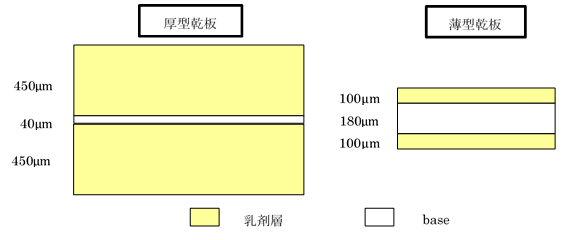
\includegraphics[clip, width=60mm]{emulsionorder.png}
            \hspace{1.6cm} (a)1枚目
          \end{center}
        \end{minipage}

        % 2枚目の画像
        \begin{minipage}{0.5\hsize}
          \begin{center}
            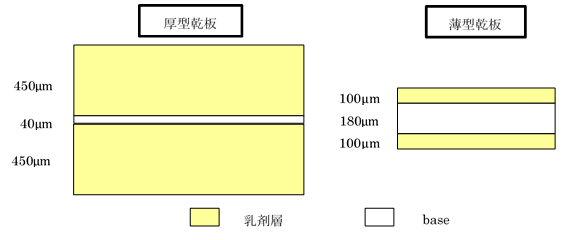
\includegraphics[clip, width=60mm]{emulsionorder.png}
            \hspace{1.6cm} (b)2枚目
          \end{center}
        \end{minipage}
    
      \end{tabular}
      \caption{画像}
      \label{fig:img}
    \end{center}
\end{figure}
\par
画像のコントラストをよくするために用いる式は以下の通りである。
図●はこの式を使用して画像にコントラスト処理を施した画像である。
図より画像の最も輝度値の明暗の幅が広がったことが分かる。
\subsubsection{ガウシアンフィルタ処理}
\begin{itemize}
    \item 撮影された画像にはノイズが記録されているので、そのノイズを消すためにガウシアンフィルタ処理により画像をぼかす。
    \item ガウシアンフィルタ処理の数式を入れる。
    \item 処理前と処理後の画像を入れる。
\end{itemize}
撮影された画像には意図していないノイズが含まれている。
機械に飛跡を認識させるために、画像を構成する1つ1つのpixelに割り当てられた輝度値情報を利用する。
ノイズにより飛跡認識に悪影響を与えないために、ガウシアンフィルタ処理をかけることで画像中のノイズを消去する。
\par
ガウシアンフィルタ処理とは、
画像中のある画素を中心に指定範囲(カーネルサイズ)内で注目画素に近いほど輝度値の平均値を計算するときの重みを大きくするように処理をかけることである。
式は次の通りである。
この式を使い、処理を実施した。
\subsubsection{画像の白黒反転}
\begin{itemize}
    \item ガウシアンフィルタ処理とコントラスト処理をかけた画像の輝度値の差分を取ることで、白黒反転の画像を作成する。
    \item 今後の画像処理のために白黒反転処理を行う。
    \item 処理前と処理後の画像&なぜ白黒反転になるのかの図を入れる。
\end{itemize}
次の二値化処理を実施するため、画像の白黒を反転させる必要がある。
ガウシアンフィルタ処理を施した画像から、コントラスト処理を施した画像の輝度値の差を取ることで白黒を反転する。
図●は画像と指定した行の輝度値を示したものである。
画像の輝度値差をとって作成した画像が図●である。
図●を見れば分かるように差分を取ることで、黒色であった部分が白色に反転した。
\subsubsection{二値化}
\begin{itemize}
    \item 白黒反転画像に対して、ある一定以上の輝度値をもつピクセルのみ残すという処理を行う。
    \item これによりある程度濃く記録された飛跡情報のみがのこるのでこのようにしている。飛跡のエネルギーが高いものは濃く記録されると言うことの図を入れた方が良いかも。
    \item 処理前と処理後の画像
\end{itemize}
図●を見ると、視野中心にある飛跡情報以外に多くのgrain、trackが記録されていることが分かる。
これらの情報は飛跡追跡を実施するのに不必要であり、飛跡の誤検出を招く恐れがある。
そこで、二値化処理により指定した輝度値以下のピクセルの輝度値をゼロにする。
これにより飛跡以外の不要な輝度値情報を消す。
\par
図●は二値化処理前後の画像とその指定した行の輝度値を示したものである。
図を見れば分かるように、二値化処理により飛跡以外の不要な輝度値情報が減少したことが分かる。
\subsection{座標変換}
\begin{itemize}
    \item affine変換について書く。
    \item 追跡の際に考える必要のある座標系について書く。
    \item それらの座標系をつなぐためにaffine変換をつかい、目的の飛跡の位置に行くことが必要である。
\end{itemize}
追跡するべき飛跡情報はDetector座標系(SSD座標系)、Grid座標系(現像前座標系)、Stage座標系(現像後座標系)の3座標系で表すことができる。
Detector座標系はSSDの検出座標系である。
Grid座標系はemulsionにbeam照射をして現像をする前の座標系である。
Stage座標系は顕微鏡で原子核乾板を観察する際の座標系である。
\par
SSDで検出された候補飛跡はDetector座標系で記録されている。
検出された候補飛跡を原子核乾板で観察するためにはDetector座標系、Grid座標系、Stage座標への変換を適切に行う必要がある。
その座標間の変換を適切に行うためにaffine変換を使用する。
\par
\subsection{自動追跡の要素技術}
\subsubsection{P-barパターンマッチ}
\begin{itemize}
    \item SSDとemulsionの位置ズレを取得するのに必要。
    \item 乾板の四隅に照射されているものを使う。(なぜP-barを使うのか、どのようにP-barが照射されているか確認する。)
    \item どのようにP-barを取得するのか(スキャンする場所等を書く)を書く。
    \item 四隅のうち3点箇所でパターンマッチがとれればズレが取得できる。(精度について書く。)
\end{itemize}
原子核乾板にはSSDとemulsionの照射時の位置差を取得するために反陽子ビームが照射されている。
照射されているのは乾板の四つ角1cm1cmの領域である。
照射されている反陽子beamの濃度は1平方センチあたり10の4乗である。
k-beamは乾板に対して10の6乗照射されており、SSDとemulsionのパターンマッチをするには密に照射されすぎているのでp-barが必要になる。
\par
角から1cmずつ内陸側に移動し、そこで5mm×5mmの領域をスキャンする。
上側乳剤層と下側乳剤層をスキャンし、baseを挟んで接続された垂直なbeamを使いパターンマッチを行う。
\par
\subsubsection{$\Xi$$^-$候補飛跡の選択}
\begin{itemize}
    \item 追跡の際に考える必要のある座標系について書く。
    \item それらの座標系をつなぐためにaffine変換をつかい、目的の飛跡の位置に行くことが必要である。
\end{itemize}
追跡するために、SSDで検出した$\Xi$$^-$候補とpl01に記録された荷電粒子飛跡の対応をつける。
先述したP-barパターンマッチにより、SSDと原子核乾板の座標の対応がついている。
SSDで検出された$\Xi$$^-$候補の位置情報と角度情報を使い、薄型原子核乾板1枚目のbase上面まで外挿する。
これにより$\Xi$$^-$候補の薄型原子核乾板1枚目のbase上面における位置がおおよそ分かる。
この薄型原子核乾板1枚目のbase上面における位置情報と角度情報を合わせてprediction(pred)とする。
\subsubsection{K$^-$beamパターンマッチ}
\begin{itemize}
    \item emulsionとemulsionの位置ズレを補正するために行う。
    \item これにより、例pl01で記録された飛跡とpl02で記録された飛跡の対応付けをする。
    \item どこをスキャンして、どのようになるのかを書く。模式図を書く。
\end{itemize}
beam照射時の上流乾板と下流乾板の位置ずれを取得するために乾板に照射されているK$^-$beamを用いてパターンマッチを行う。
\subsubsection{表面認識}
\begin{itemize}
    \item 乳剤層と非乳剤層の境界面を取得するために行う。
    \item 乾板中の位置における輝度値の違いを示す。
\end{itemize}
\subsubsection{荷電粒子飛跡追跡}

\newpage
\section{E07乾板における開発プログラムでの追跡実績}

\newpage
\section{まとめ}

\section*{付録}
\addcontentsline{toc}{section}{付録}
これは付録でいいかな???
原子核乾板中に記録されたHyper核eventを解析するためには記録されている原子核乾板の密度が重要になる。
記録された飛跡の飛程からエネルギーを算出する際に乾板の密度が必要になるからである。
現在核種が一意に決定されている'NagaraEvent'の解析にはevent付近に記録されたα崩壊飛跡を50例使用し、乾板の密度を計算して○.○○とした。
\par
表○はNagaraの各trackの長さ、角度を示している。
trackの長さ、角度が一定で、原子核乾板の密度を変化させたときBΞがどれだけ変化するかを確認した。
図●はその変化を示している。
図から分かるように密度の変化によってBΞは大きく変化する。
そのため原子核乾板の密度を正確に求めること、密度が解析において非常に重要であることが分かる。
\par
図を入れる。
\par


\section*{謝辞}
\addcontentsline{toc}{section}{謝辞}
ああああああああああああああああああああああああああ
\begin{thebibliography}{99}
\bibitem{Nagara} 「Double-$\Lambda$Hypernuclei observed in a hybrid emulsion experiment」PHYSICAL REVIEW C NUCLEAR PHYSICS Vol.88,No.1, July 2013
\bibitem{Nagara2} 「”NAGARA event”が語る相互作用―KEK-PS E373 ダブルハイパー核実験―」仲澤和馬(岐阜大学)、高橋仁(京都大学)、PS-E373 共同実験グループ 高エネルギーニュース Vol.20 No.5 p.206 2002
\bibitem{takusann} 学位論文「大規模実験用高性能原子核乾板OPERA Filmの開発」第四章 Refresh処理 名古屋大学大学院理学研究科素粒子宇宙物理学専攻F研究室 中村琢 著(2005年)
\end{thebibliography}
\end{document} 